\chapter{Semantic Web Basics} \label{ch:briefintrosemanticweb}

Ontology is the philosophical study of the nature of being, existence, or reality. In the context of the Semantic Web, ontology refers to a formal specification of concepts, relationships, and categories of a particular domain or knowledge base. Ontology allows the creation of a shared understanding of a particular domain, enabling machines to interpret and reason about data more effectively. Ontology is essentially about “what is everything”. It is about how we as humans mark our existence, and how we preserve and add to our knowledge base for the generations to come.

Ontology inspires people in computer science how we can store and exchange information more efficiently by building an internet based knowledge base. The solution is called the semantic web. An internet powered by semantic web (together with other technologies) defines web 3.0.

\section{Web of Data}

The Internet, as we call it today, is a technology that enables information exchange between machines, as well as between machines and human beings. With the power of the Internet, humans can obtain the information they need from remote servers, databases, or knowledge bases.

Initially, this information exchange was difficult, and professional computer skills were required to operate the Internet and its human-machine interface. Nowadays, everyone can access the Internet by just using a graphical browser. Public knowledge bases like Wikipedia make obtaining information much easier.

Following this trend, AI knowledge bases combined with human-readable semantic web technologies such as RDF and OWL, will become more and more popular and provide additional help for knowledge transfer and sharing.

\subsection{Web 1.0 and 2.0}

In the age of Web 1.0, knowledge was stored on individual servers, often in a static manner. Users could open a browser and check the knowledge as it was presented in the form designed by the server owner. It was essentially a one-way data transmission. The experts provide information, and the ordinary users consume the information.

In the age of Web 2.0, thanks to more advanced communication technologies, users can interact with web service providers. They can search and filter data from the servers and even upload their own data to the servers and share it with others. The Internet became easier and more flexible to use for information exchange, and data transfer became bidirectional. Ordinary users are both providers and consumers of information on the Internet. Databases are used in the backend which allows the user to push and pull data from the server.

Web 2.0 is useful but still far from perfect, especially given the background of industry 4.0 and data-driven everything.

One of the biggest challenges that we encounter with Web 2.0 is how to quickly locate the information we want hidden among the vast amount of data on the Internet. Among all the information available, which is important, and which is redundant? Humans have contextual knowledge and experience to solve the problem, but it will take forever.

Keyword search engines are widely used in the Web 2.0 framework, and it is the main method one can rely on when pulling information from the Internet. Keyword search engines may struggle with polysemous, synonyms, unintended personalizing, and implicit information from pictures.

Today most of the information on the Internet is stored in HTML format. HTML tells the contents links to the information, but not the meaning behind it. It is difficult for a machine to understand the meaning of the information from HTML files. As will be introduced later, this potentially makes it difficult for a machine to retrieve data efficiently.

\subsection{Web 3.0}

The ultimate goal of Web 3.0 is to allow more efficient information search and transfer using the Internet, given the vast amount of existing data hosted on distributed servers and sensors.

In order to search, exchange, and abstract useful information from distributed sources in an efficient manner, there are at least two things we can do:

\begin{itemize}
  \item Let the machine do the job. The AI should be smart enough to precisely capture what the user wants and get back to him with useful and accurate results.
  \item Make the information stored on the Internet more readable for both humans and machines, i.e., make the information semantic (meaningful).
\end{itemize}

The above forms the fundamentals of Web 3.0. The first point leads to smart chatbot, and the second to semantic web.

Web 3.0 relies on advanced data storage, data searching, and data processing technologies. We need to develop powerful AI so that it can interpret the user demands, search for useful information in its knowledge base efficiently, and finally come back with a human-readable answer. For that, we need advanced natural language processing techniques, and efficient (and potentially online) AI training techniques to keep the sophisticated knowledge base up to date.

In addition, we need to formally express the semantics (meanings) of the information for everything put online. This helps both humans and machines to interpret information and decide whether it is useful. This introduces the concept of the semantic web, which is a significant aspect of Web 3.0. In fact, semantics are so important that they are often considered synonymous with Web 3.0, although the broader vision of Web 3.0 includes other features as well.

Distributed storage has both advantages and disadvantages. On one hand, it provides higher resilience against data loss. On the other hand, it adds difficulty to the searching and collecting of information. Technologies like IPFS, blockchain, and distributed databases are being used to address these challenges.

This notebook focuses on the technologies used in semantic web, some of which such as RDF and OWL have already been implemented. We will see how we can use semantic web to collect and organize information, and from where how we can create a knowledge base for both humans and AI.

\subsection{Semantic Web Vision}

How to make contents on the Internet meaningful to machines?

Recall the 2 bullet points in the previous section. We always have the choice to use AI with powerful natural language processing capability. This of course relies on technologies in machine learning. We need to design ANN models that can be easily massively trained and it needs to be able to capture long text that humans usually use. With the development of transformer, this is becoming promising. There is another challenge though, which is that the knowledge base formed by AI is a black box, and cannot be interpreted by other machines with a different framework. In other words, you cannot build a knowledge base with AI and use it everywhere without any tuning. Transfer learning and knowledge distillation may help, but they also have constraints.

In the semantic web vision, we mainly focus on another approach, which is **annotating explicit semantic metadata to the existing content**. The semantic metadata shall be encoded the meaning of the content in a machine-readable way.

Semantic web approach is complementary with AI approach. It has some advantages:
\begin{itemize}
  \item The knowledge is more transparent, unlike AI where the knowledge is hidden in the ANN as a black box.
  \item The knowledge is reusable and scalable in a easier way than AI knowledge base which relies on knowledge distilling (reuse) and transfer learning (rescale).
  \item RDF and OWL, the tools we use to organize and store knowledge in semantic web, are more reader-friendly for both humans and machines.
\end{itemize}

Many research facilities and organizations have tried building semantic web for either global or specific domains. An example is DBPedia \textit{dbpedia.org}. The goal of DBPedia is to create something like Wikipedia, but semantic.

\subsection{Semantic Web Stack} \label{subsec:semanticwebstack}

A commonly seen semantic web stack looks like Fig. \ref{fig:semanticwebstack}. It is a summary of components and tools used in building a semantic web.

\begin{figure}[htbp]
	\centering
	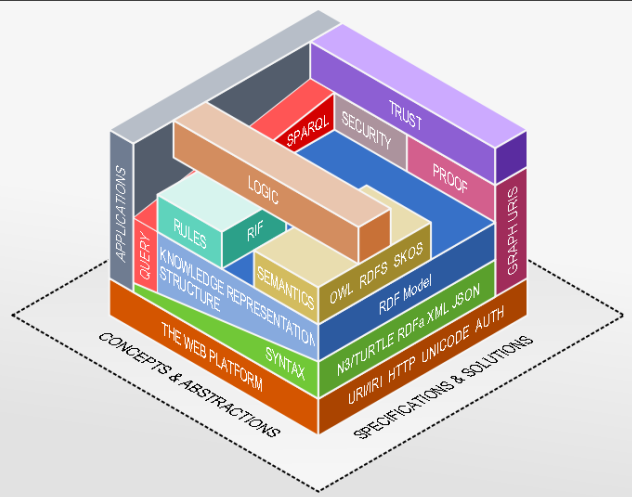
\includegraphics[width=0.8\textwidth]{./chapters/ch-semanticwebbasics/figures/semanticwebstack.png}
	\caption{Semantic web stack introduced in \cite{semanticwebstack}.}
	\label{fig:semanticwebstack}
\end{figure}

In the very bottom is the platform that hosts everything. It is also the representation of all the existing knowledge. Uniform Resource Identifier (URI) is the “address” that can be used to identify a information source. It can be in the form of an URL to the web page that introduces an item. For example, ``About: Semantic Web (dbpedia.org)'' \textit{dbpedia.org/page/Semantic_Web} is the URL to the defination of semantic web in DBPedia. The web page represents semantic web as part of the existing knowledge (this web page is not stand alone though, as later we will see that it links to other sources using linked data).

N3, TURTLE, XML, JSON and Resource Description Framework (RDF) model are used to organize and store data. N3, TURTLE, XML and JSON is the syntax of the text, while RDF demonstrates the knowledge representation structure. The following is an example of using semantic web stored in TURTLE. Only the first few lines are given. Details to the syntax are introduced in later chapters.

\begin{lstlisting}
@prefix dbo:	<http://dbpedia.org/ontology/> .
@prefix dbr:	<http://dbpedia.org/resource/> .
dbr:Semantic_web	dbo:wikiPageWikiLink	dbr:Semantic_Web ;
	dbo:wikiPageRedirects	dbr:Semantic_Web .
dbr:Knowledge_management	dbo:wikiPageWikiLink	dbr:Semantic_Web .
dbr:Intelligent_agent	dbo:wikiPageWikiLink	dbr:Semantic_Web .
dbr:Wiki_software	dbo:wikiPageWikiLink	dbr:Semantic_Web .
dbr:List_of_Brown_University_alumni	dbo:wikiPageWikiLink	dbr:Semantic_Web .
dbr:NitrosBase	dbo:wikiPageWikiLink	dbr:Semantic_Web .
dbr:Arabic_Ontology	dbo:wikiPageWikiLink	dbr:Semantic_Web .
dbr:Semantic_Web_Stack	dbo:wikiPageWikiLink	dbr:Semantic_Web .
dbr:Giant_Global_Graph	dbo:wikiPageWikiLink	dbr:Semantic_Web .
dbr:Computational_semantics	dbo:wikiPageWikiLink	dbr:Semantic_Web .
dbr:Deborah_McGuinness	dbo:wikiPageWikiLink	dbr:Semantic_Web ;
	dbo:academicDiscipline	dbr:Semantic_Web .
\end{lstlisting}

Information is tagged in RDF. RDF, together with RDF Schema (RDFS) provides limited semantics, and it created a foundation of semantic that allows Web Ontology Language (OWL) to build more complicated semantics on top of it, such as adding rules on restrictions and disjoint classes. In this sense, OWL is an extension of RDF.

SPARQL (SPARQL Protocol and RDF Query Language) is the standard query language for querying and manipulating RDF data on the Semantic Web. It allows users to search, retrieve, and modify information stored in RDF format.

The syntax of SPARQL is similar to SQL, as both are query languages designed for structured data. SPARQL was influenced by SQL, and many concepts in SPARQL have counterparts in SQL, such as SELECT, WHERE, GROUP BY, and ORDER BY. However, the backend technologies differ largely.

SQL is designed to query and manipulate data stored in relational databases, which are based on tables with rows and columns. On the other hand, SPARQL is designed for querying and manipulating RDF data, which is based on graphs with nodes and edges. In SPARQL, you work with RDF triples and graph patterns, and use operations such as graph pattern matching to find data that satisfies specific conditions. Their interfaces look similar, but the backend technologies differ largely.

An example of a knowledge base using RDF/RDFS/OWL is given below, together with a SPARQL query.

\begin{mdframed}

\vspace{0.1in}
{\centering \textbf{Example: Knowledge Base on Animals}}
\vspace{0.1in}

The following examples demonstrates how to use RDF/RDFS and OWL to create a small knowledge base about animal. The example is provided by \textit{ChatGPT-4}.

\vspace{0.1in}
\noindent \textbf{RDF/RDFS}
\vspace{0.1in}

\begin{lstlisting}
@prefix rdf: <http://www.w3.org/1999/02/22-rdf-syntax-ns#> .
@prefix rdfs: <http://www.w3.org/2000/01/rdf-schema#> .
@prefix ex: <http://example.org/> .

ex:Animal rdf:type rdfs:Class .

ex:Mammal rdf:type rdfs:Class ;
    rdfs:subClassOf ex:Animal .

ex:Reptile rdf:type rdfs:Class ;
    rdfs:subClassOf ex:Animal .

ex:hasLegs rdf:type rdf:Property ;
    rdfs:domain ex:Animal ;
    rdfs:range rdfs:Literal .

ex:Dog rdf:type rdfs:Class ;
    rdfs:subClassOf ex:Mammal .

ex:Lizard rdf:type rdfs:Class ;
    rdfs:subClassOf ex:Reptile .

ex:Max rdf:type ex:Dog ;
    ex:hasLegs 4 .

ex:Lizzy rdf:type ex:Lizard ;
    ex:hasLegs 4 .
\end{lstlisting}

In this example, we used RDF and RDFS to:
\begin{itemize}
  \item Define classes (Animal, Mammal, Reptile, Dog, and Lizard)
  \item Define a property (hasLegs)
  \item Set the domain and range of the property
  \item Create subclass relationships (Mammal and Reptile are subclasses of Animal; Dog is a subclass of Mammal; Lizard is a subclass of Reptile)
  \item Define individuals (Max and Lizzy) and their properties
\end{itemize}

\vspace{0.1in}
\noindent \textbf{OWL}
\vspace{0.1in}

\begin{lstlisting}
@prefix rdf: <http://www.w3.org/1999/02/22-rdf-syntax-ns#> .
@prefix rdfs: <http://www.w3.org/2000/01/rdf-schema#> .
@prefix owl: <http://www.w3.org/2002/07/owl#> .
@prefix ex: <http://example.org/> .

ex:hasParent rdf:type owl:ObjectProperty ;
    rdfs:domain ex:Animal ;
    rdfs:range ex:Animal .

ex:hasChild rdf:type owl:ObjectProperty ;
    owl:inverseOf ex:hasParent .

ex:isWarmBlooded rdf:type owl:Class ;
    rdfs:subClassOf ex:Animal .

ex:Mammal rdfs:subClassOf ex:isWarmBlooded .

ex:Reptile owl:disjointWith ex:isWarmBlooded .

ex:Max ex:hasParent ex:Buddy .

ex:Buddy rdf:type ex:Dog ;
    ex:hasLegs 4 .
\end{lstlisting}

In this example, we used OWL to:
\begin{itemize}
  \item Define object properties (hasParent and hasChild)
  \item Specify an inverse relationship between properties (hasParent and hasChild)
  \item Define a new class (isWarmBlooded) and set it as a superclass of Mammal
  \item Specify a disjoint relationship between Reptile and isWarmBlooded
  \item Define a new individual (Buddy) and his properties
  \item Specify a relationship between individuals (Max and Buddy)
\end{itemize}

In this demonstration example, RDF and RDFS provided the basic structure and hierarchy for the knowledge base, while OWL added more expressivity by defining complex relationships, additional semantics, and constraints.

Finally, the above knowledge base can be queried by SPARQL as follows.

\begin{lstlisting}
PREFIX ex: <http://example.org/>

SELECT ?mammal
WHERE {
  ?mammal rdf:type/rdfs:subClassOf* ex:Mammal .
}
\end{lstlisting}

\end{mdframed}

SPARQL query is not user-friendly. Commercialized semantic web applications such as WolframAlpha \textit{wolframalpha.com} often provides a ``search bar'' with limited NLP capability to make the searching of the semantic web easier. It is worth mentioning that although this searching engine may look like chatbot at a first glance, their underlying information source and techniques differently largely. See ChatGPT-4's comments as follows.

\begin{mdframed}

\textbf{I understand that chatbot like you works differently compared with these engines such as WolframAlpha. While their knowledge comes from semantic web, your knowledge comes from years of training using natural-language-written books and articles. Am I right?}

Yes, that's correct. As an AI language model, I am based on the GPT-4 architecture developed by OpenAI. My primary source of knowledge comes from the vast amount of text data that I have been trained on, which includes books, articles, and other documents written in natural language. My training data consists of diverse sources and covers a wide range of topics up to my knowledge cutoff date in September 2021.

Unlike search engines like WolframAlpha or tools that rely on the Semantic Web, my knowledge representation and understanding are not based on formalized structures like RDF or OWL. Instead, I analyze and generate text based on patterns and relationships learned from my training data.

This approach has some advantages and limitations. On the one hand, I can provide more human-like, natural language responses and can generate text on a wide range of topics, even if I have not been specifically trained on a particular domain. On the other hand, my understanding of the underlying structure and semantics of the data may be less precise than that of systems that use formal knowledge representation languages like RDF or OWL.

In summary, chatbots like me and engines like WolframAlpha operate differently in terms of their knowledge sources and representation, but both approaches can be useful for providing information and answering questions in their respective domains.
\end{mdframed}

Chatbot and semantic web can work together. Chatbot is used to provide a human interface and basic domain knowledge, while the semantic web provides up-to-date precise informative facts.

\subsection{Semantic Web Limitations and Challenges}

It is worth mentioning that though semantic web is powerful, building semantic web can be challenging because it requires a lot of human labor. As of 2023, the majority of web sites and applications have not yet embraced the full potential of the semantic web, some of which only partially adopt semantic web concepts or technologies.

ChatGPT-4 comments on the current status of semantic web applications as follows.

\begin{mdframed}
The semantic web has made significant progress since its inception, but it hasn't been adopted as widely as initially envisioned. Many organizations, research institutions, and some large corporations have adopted semantic web technologies for specific use cases, such as knowledge management, data integration, and domain-specific applications. However, the majority of websites and web applications have not yet embraced the full potential of the semantic web.

That being said, some aspects of the semantic web have become popular and are widely used:

\begin{enumerate}
  \item Structured data markup: Many websites use structured data markup, such as schema.org, to provide additional semantic information about their content. This helps search engines like Google to better understand the content and present it more effectively in search results. While not the full realization of the semantic web vision, this is a step towards making the web more machine-readable.
  \item Linked Data: The concept of Linked Data, which is closely related to the semantic web, has gained some traction. Linked Data is a method of publishing structured data on the web so that it can be interlinked and easily accessed by machines. Examples include DBpedia, Wikidata, and various governmental and organizational datasets.
  \item Research and academia: The semantic web has been a popular research topic in academia, with numerous conferences, workshops, and publications dedicated to its development and application. This has led to the development of various tools, algorithms, and methodologies that have been adopted in specific domains.
  \item Domain-specific applications: Some industries and sectors, such as healthcare, life sciences, and digital libraries, have adopted semantic web technologies to manage their complex data and facilitate data integration and interoperability.
\end{enumerate}

While the semantic web has not been adopted as widely as originally anticipated, its core ideas and technologies have had an impact on various areas of the web, and its principles continue to influence the development of new standards and technologies. It's possible that as AI and machine learning technologies continue to advance, there will be renewed interest in the semantic web and its potential to facilitate machine understanding of web content.

There are several challenges that have contributed to the semantic web not being embraced to its full potential:

\begin{enumerate}
  \item Complexity: Semantic web technologies, such as RDF and OWL, can be complex and difficult to understand for many web developers, especially those without a background in knowledge representation, logic, or artificial intelligence. This complexity can act as a barrier to adoption.
  \item Lack of incentives: Many website owners and content creators may not see immediate benefits or incentives for adopting semantic web technologies. Implementing semantic annotations and structured data can be time-consuming and resource-intensive, especially for smaller organizations or individuals without dedicated technical teams.
  \item Incomplete coverage: The vision of the semantic web relies on a large amount of high-quality, machine-readable data being available. However, not all websites provide structured data or semantic annotations, which limits the effectiveness of semantic web applications and discourages further adoption.
  \item Ontology development and maintenance: Creating and maintaining ontologies, which are key components of the semantic web, can be a complex and time-consuming task. Achieving consensus on common vocabularies and ontologies across different domains and stakeholders can also be challenging.
  \item Scalability and performance: Semantic web technologies need to handle large-scale data processing and reasoning tasks, which can be computationally expensive. Some traditional semantic web tools and algorithms may not scale well for big data or real-time applications.
  \item Privacy and security concerns: The semantic web promotes data sharing and integration, which can raise privacy and security concerns for both individuals and organizations. Ensuring that sensitive data is protected while still enabling the benefits of the semantic web can be a challenging balance to strike.
  \item Competition from other technologies: Other technologies and approaches, such as keyword-based search engines, relational databases, and machine learning, have continued to evolve and provide effective solutions for many data management and retrieval tasks, which may have reduced the urgency for adopting semantic web technologies.
\end{enumerate}

Overcoming these challenges will require continued research, development, and collaboration among researchers, developers, and stakeholders. As new tools, algorithms, and techniques are developed, and as the importance of machine understanding of data increases, there may be renewed interest in and adoption of the semantic web.

Despite the challenges in the widespread adoption of the semantic web, its core ideas and principles have had a significant impact on various fields, especially in the development of domain-specific knowledge bases and applications. The concepts of ontology, structured data, and linked data have inspired and facilitated numerous projects and use cases, such as:

\begin{enumerate}
  \item Domain-specific ontologies: The development of domain-specific ontologies has allowed organizations and researchers to model and represent complex knowledge structures and relationships in their respective fields. Examples include the Gene Ontology (GO) in the life sciences, the CIDOC Conceptual Reference Model (CRM) in cultural heritage, and the Financial Industry Business Ontology (FIBO) in finance.
  \item Data integration and interoperability: Semantic web technologies have been instrumental in integrating and sharing data across different systems, platforms, and organizations. By utilizing shared ontologies and vocabularies, data can be mapped and linked more easily, enabling better interoperability and reducing the need for manual data reconciliation.
  \item Knowledge management and discovery: Semantic web technologies have been used to build intelligent knowledge management systems that can infer new information and discover hidden relationships by reasoning over structured data. This can help organizations make better decisions, discover new insights, and optimize their processes.
  \item Personalization and recommendation systems: By incorporating semantic web technologies and leveraging domain-specific knowledge bases, recommendation systems can provide more accurate and personalized suggestions based on users' preferences, behaviors, and the underlying relationships between items.
  \item Natural language processing and AI: The ideas behind the semantic web have inspired research in natural language processing (NLP) and AI, as they both strive to enable machines to better understand and process human-generated content. Semantic web technologies can be used to enrich NLP tasks and enhance AI models with structured knowledge.
\end{enumerate}

While the semantic web has not yet reached its full potential, its principles and concepts continue to influence and inspire the development of new technologies and applications, especially in the context of building domain-specific knowledge bases and fostering knowledge sharing and discovery.

\end{mdframed}

With the population of LLM powered chatbot and IoT as part of Industrial 4.0, things might change. It has been extremely difficult to check the correctness and consistency of the existing data bases (both structured and unstructured) due to the large volume of data, let along converting them into semantic web. With the help from chatbot, the checking and conversion might be automated. In addition, as Industry 4.0 and IoT technologies continue to advance, the amount of structured data generated will increase significantly. This structured data can be a valuable resource for building semantic web applications more easily and effectively. A knowledge base that combines semantic web and chatbot might become a future standard. ChatGPT-4 comments as follows.

\begin{mdframed}
In the future, the combination of AI chatbots and semantic web technologies could become a powerful standard for handling various tasks. AI chatbots would serve as the natural language interface for users, providing basic knowledge and understanding of context, while the semantic web would provide accurate, up-to-date, and domain-specific data.

Integrating AI chatbots with SPARQL or other semantic web querying capabilities can enable them to search, analyze, and interpret structured data more effectively. This way, chatbots could provide users with more precise and relevant information based on the available structured data.

Such a combination of technologies would not only make it easier for users to access and interact with the vast amount of structured data, but it would also enable AI systems to better understand the context and semantics of information, leading to improved performance and more accurate results.
\end{mdframed}

\section{Ontology} \label{sec:ontology}

Ontology has very rich meanings with both philosophy and semantic web perspective.

\subsection{Philosophy Perspective}

Knowledge is the intersect of ground truth and human beliefs, i.e., it is the truth that humans know of being truth. Ontology is a way of communicating knowledge.

In the context of philosophy, ontology discusses the meaning of an object “exists”, how objects can be categorized, and how objects relate to each other. Ontology mainly discusses the following questions:

\begin{itemize}
  \item What is existence?
  \item What are the fundamental categories of existence?
  \item What does it mean for something to exist or not exist?
  \item What types of entities exist, and what is their nature?
  \item What is the nature of abstract entities like numbers, properties, and relations?
  \item How do different entities relate to each other and interact?
  \item Can something exist independently of our perception or thought?
\end{itemize}

The discussion of these questions can be traced back to BC300 and earlier. Aristotle defined a system to structure and reasoning knowledge. The famous Aristotelian logic “major premise + minor premise -> conclusion” is in fact a standard and systematic way of reasoning unknown from knowledge. Aristotelian logic is an important tool of ontology, and it inspires how we build semantic web, even after these many years.

The first idea of creating a machine to categorize things came in 1200s. The first idea of creating a “universal precise language” to record knowledge was proposed in 1600s.

\subsection{Semantic Web Perspective}

In the context of the Semantic Web, an ontology is a formal, machine-readable representation of a specific domain's concepts, their properties, and the relationships between them. It serves as a shared vocabulary (unlike natural language, which is often ambiguous) for describing and reasoning about the knowledge within that domain. In practice, RDF/RDFS and OWL can be used to express the ontology.

The followings are defined in RDF/RDFS and OWL.

\begin{itemize}
  \item Class. Classes are used to represent components and models. It represents a concept. It is an abstraction of objects sharing some similarities.
  \item Attribute. Attributes are used to describe classes.
  \item Relations. Relations are special attributes whose values are objects of (other) classes.
  \item Constraints. The attributes of classes might be restricted. For example, a class may have an multiple attributes of similar kind (consider a person has many houses). A class may not have two attributes at the same time (consider a person cannot be man and woman at the same time).
  \item Instance. An instance is an individual of an ontology. For example, “John is a person”, where “person” is a class.
\end{itemize}

\subsection{Knowledge and Logic} \label{subsec:knowledgeandlogic}

Different knowledge frameworks and logic types are briefly introduced in this section. They are covered in more details in later sections, including Section \ref{sec:logic} for logic frameworks, logic equivalence, and logic reasoning, Section \ref{sec:dlalc} for description logic (DL) and attributive language with complement (ALC), and Section \ref{sec:owl} for OWL.

Knowledge should be stored in such a way that new knowledge can be derived from existing knowledge, and there should be a standardized way of deriving new knowledge from existing knowledge. This introduces the important concept of logic.

Propositional logic is the fundamental of the logic that we know of today. In propositional logic, knowledge is represented by simple facts (simple proposition), and facts connected with  AND, OR, NOT, IF THEN, IF AND ONLY IF (compound proposition).

First-order logic (FOL) is the most commonly used logic as of today. In FOL, quantifiers and logic connectives are introduced, including universal quantification $\forall$, existential quantification $\exists$, conjunction, disjunction and negation. A formal way of representing logic expressions are defined. For example, using the following to represent ``all humans are mortal''
\begin{eqnarray}
\forall x \left(\textup{Human}(x) \rightarrow \textup{Mortal}(x)\right) \nonumber
\end{eqnarray}
where $\textup{CLASS}(x)$ is equivalent of a proposition ``$x$ belongs to CLASS'', which can be either true or false. The above proposition says ``for any item, if that it belongs to human is true, then that it belongs to mortal must be true''. Given the current biology development, this proposition is still true.

Description logic (DL) is a subset of the first-order logic. DL is specifically designed to represent and reason about ontologies and their concepts, relations, and instances. It focuses on capturing the semantics of structured knowledge with a restricted set of constructs and reasoning capabilities. The idea of semantic web builds on top of DL.  Some key features of DL are:
\begin{itemize}
  \item Defining classes and subclasses
  \item Defining properties (roles) and their domain and range:
  \item Defining restrictions on classes
  \item Using existential and universal quantifiers
\end{itemize}
Semantic web is essentially an implementation of DL on computers. As can be seen later, many tools used in semantic web, such as RDF/RDFS and OWL, are essentially practicing DL in a machine-readable way.

Attributive language with complement (ALC) is one of the ways to describe a simple DL, and it forms an important subset of OWL which enables ontology in semantic web. Understanding ALC is helpful with learning OWL in later sections. A brief introduction of ALC is given below.

``Concept'' (corresponding with class in RDF/RDFS) and ``role'' (corresponding with property in RDF/RDFS) are introduced. Top concept and bottom concepts are defined. Each property is associated with a range, which is a basically a set of values that the property can take. Concepts and roles are atomic types defined in ALC.

Constructors are used to describe ranges and their relationship with a property. Conjunction/Intersection, disjunction/union and negation/complement of a range are defined. Existential and universal quantifiers are defined. For example, \verb|\forall R.C| can be used to say that all attributes of property type ``R'' should stay within range ``C''. Similarly, \verb|\exists R.C| means that there should be at least one attribute of property type ``R'' whose value stays within range ``C''.

Class relations are defined. Commonly used class relation constructors are inclusion (to describe sub class) and equality (to assign class), union, intersection, complement, etc.

Knowledge is expressed in two formats, either being terminological knowledge, or assertional knowledge. As a terminological knowledge example, we can define a teacher as
\begin{lstlisting}[mathescape=true]
	Teacher $\equiv$ Person $\wedge$ $\exists$ HasStudent.Student $\wedge$ $\exists$ Teaches.Class
\end{lstlisting}
which translates to ``a teacher is a person, and has relationship HasStudent with at least one Student element, and has relationship Teaches with at least one Class element, and ``Person'', ``Student'', ``Class'' are classes, ``HasStudent'', ``Teaches'' properties, defined in RDF/RDFS. There are people who teaches only tutorials but not classes. To include them into the teacher class, consider using
\begin{lstlisting}[mathescape=true]
	Teacher $\equiv$ Person $\wedge$ $\exists$ HasStudent.Student $\wedge$ ($\exists$ Teaches.Class $\vee$ $\exists$ Teaches.Tutorial)
\end{lstlisting}
It can be seen that with terminological knowledge, a lot of restrictions and rules can be added when defining a class.

As an assertional knowledge, we can state an instant or a sub class to be of Teacher as follows.
\begin{lstlisting}
	Teacher(Peter)
	Teaches(Peter, LinearAlgebra)
\end{lstlisting}

All the above can be translated into OWL, which largely enriches the capability of RDF model building relations and restrictions among classes. More details are given in later sections.


\subsection{Ontology Types and Categories}

There are different layers of ontology. The higher the layer, the more general it is. The lower the layer, the more specific it is to a particular research domain, a particular application, or even a particular task. An example is given in Fig. \ref{fig:ontologylevel}. In practice, there might not be a clear boundary between two adjacent ontology layers.

\begin{figure}[htbp]
	\centering
	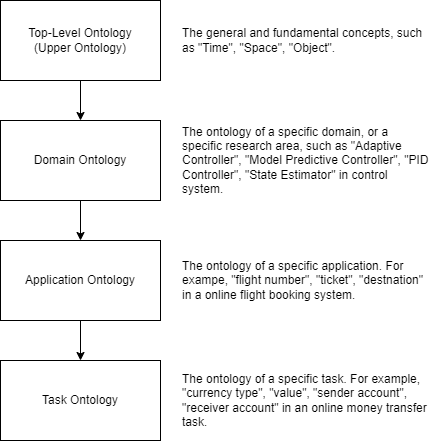
\includegraphics[width=0.8\textwidth]{./chapters/ch-semanticwebarchitecture/figures/ontologylevel.png}
	\caption{A demonstration of ontology level.}
	\label{fig:ontologylevel}
\end{figure}

Lower-layer ontology can import concepts and knowledge from the upper-layer ontology. If needed, it can modify the imported concepts.

Other ways of leveling ontology include using the expressiveness. The ``light-weight'' ontology is informal, less semantic, and supports less comprehensive logic. The ``heavy-weight'' ontology, on the other hand, is formal, more semantic, and supports more comprehensive logic and reasoning up to first-order logic. The vocabulary also grows with the ontology complexity.

\section{Logic} \label{sec:logic}

Logic and logical expression are by themselves a research area. Details on logical expression is not included in this section. Only a brief scratch is given.

Humans are good at deriving new knowledge from semantically defined existing knowledge. The tool that enables this is the logic inference. Logic is briefly introduced in this section. Logic helps to distinguish between truth and lie, so that we can accept truth and reject lie.

The idea ``formal logic'' systematically defines logic reasoning methods and procedures to automate logic inference. Logic inference engines or reasoners are used to automate this process of making logical conclusions based on the given knowledge.

\subsection{Syntax and Semantics}

We use ``syntax'' to represent ``semantics''. Syntax is just symbols without meaning that comes naturally. We humans give meaning to the syntax. The meaning of the syntax is its semantic.

Consider the following example. This is a piece of code written in Python. As anyone who has decent Python programming experience, the behavior of the code can be easily spotted, or even emulated in our brain. However, what is the semantics behind this syntax?
\begin{lstlisting}
ax = []
for i in range(20):
	if i<=1:
		ax.append(i)
	else:
		ax.append(ax[i-1]+ax[i-2])
\end{lstlisting}

When considering the semantic understanding of the simple Python script above, it's interesting to note the differences between a Python interpreter, an AI model, and human cognition.

The Python interpreter is essentially syntax-driven. When it executes a script, it follows the provided instructions one by one without any broader understanding or anticipation of the results. In the context of our Fibonacci series, the interpreter doesn't recognize that it's generating a famous mathematical sequence or why that sequence might be important or interesting. It simply follows the rules of the script, calculating and outputting each number in the series as instructed.

On the other hand, an AI model like GPT-3 does possess a level of semantic understanding, but it's quite different from that of a human. Through training on a diverse range of internet text, it has learned to associate the Python script for generating a Fibonacci series with the mathematical concept of the Fibonacci sequence. This understanding is not innate but rather a result of recognizing patterns in the data it was trained on. When asked about the script, it can provide a summary or explanation based on its learned associations, including the name of the series, and the purpose of each line of the code. It follows what it has been trained on.

Finally, there's the human level of semantics, which is by far the most advanced and intuitive. Not only can a human understand the Python script and the concept of the Fibonacci series, they can also infer its broader mathematical properties, such as its relation to the golden ratio, and its general behavior. Humans can understand that the series will converge to the golden ratio not only when starting with 0 and 1, but with any two initial positive integers. This level of understanding is a combination of learned knowledge, pattern recognition, and the ability to extrapolate or generalize from existing information.

One of the goals of semantic web is to enable machine to understand the semantic as much as possible.

The semantics can be categorized into different types.
\begin{itemize}
  \item Intentional semantics refer to the information that the producer of the information wants others to interpret, usually in natural language.
  \item Formal semantics refer to expressing the semantic in a formal language.
  \item Procedural semantics refer to the meaning of a programming language expression.
  \item Model-theoretic semantics refer to the interpretation of natural languages by identifying meaning with an exact and formally defined model.
\end{itemize}
In the context of logics, model-theoretic semantics are the main interest of study.

\subsection{Logical Expression}

Any logic consists of a set of statements $S$ and an entailment relation $\vDash$ (this can be an element or a set; in this example just take it as an element for simplicity). A logic
\begin{eqnarray}
L:= (S, \vDash) \nonumber
\end{eqnarray}
shall claim $\Phi\subseteq S$ and $\phi \in S$, where $\phi$ is a logical consequence of $\Phi$. If two logical assertions satisfy $\Phi \vDash \Psi$ and $\Psi \vDash \Phi$, then they are logically equivalent $\Phi \equiv \Psi$.

Interpretation ($I$) and formula ($F$) are two very important terms in logic expression. Interpretation is a formal construct that defines the meaning of a symbol in a formal language. For example, in the ontology of people, an interpretation can map an instance symbol, such as ``Alice'', to an actual person in the real world, and class symbol ``Person'', to the concept of a human being, etc.

Formula, on the other hand, is a statement formulated by string of symbols from a formal language. It can be a rule, or an assertion, trying to represent some fact. For example, a formula can be ``Alice hasSibling Bob''. Is it true or false? This depends on the interpretation. If ``Alice'' and ``Bob'' are indeed mapped to two siblings, and the relation ``hasSibling'' is literally what we understand it, then it is true. 

Here is another example. Consider ``10 is greater than 5''. Intuitively, this is a universal truth. But in fact, from the interpretation and formula relationship perspective, this also depends on the interpretation. It really depends on what ``10'' and ``5'' map to. If ``10'' and ``5'' are interpreted as numerical quantities and ``is greater than'' as the standard numerical greater-than relation, then it is true. However, if ``10'' and ``5'' are interpreted as amounts of debt and ``is greater than'' as a relation indicating ``is a better trader than'' (with less debt being better), then it would be false under this interpretation.

Given a formula $F$ alone, we cannot tell whether it is true or false. It is meaningful only if we discuss it with the interpretation $I$ also given. For those interpretations that make the formula true, we call them the model of the formula, and we can denote $I(F)$ or $I \vDash F$, which read as ``I models F'' or ``I satisfies F''. Different interpretations of the same symbols can lead to different conclusions. With the above, it is possible to express FOL using formal language. For example, ``all kids love icecream'' can be represented by
\begin{eqnarray}
  \forall X: \textup{Child}(X) \rightarrow \textup{lovesIcecream}(X) \nonumber
\end{eqnarray}

Multiple formulas can be grouped into a theory ($T$), which can be used interchangeably with F. A theory can be treated as a knowledge base.

\subsection{Logical Equivalence}

If two formula hold the same true and false value under the same interpretation, i.e., $F \vDash G$ and $G \vDash F$, then $F$ and $G$ are logically equivalent. The proof of logical equivalence can be done using the truth table.

There is a huge table of logical equivalence formulas. The proof of the formulas is not given here. Commonly seen equivalence is given in Table \ref{tab:logicalequivalence}.

\begin{table}
	\centering \caption{Numerical calculations.} \label{tab:logicalequivalence}
	\begin{tabularx}{\textwidth}{llX}
		\hline
		Statement & Equivalent & Comment \\
		\hline
		$\neg \neg p$ & $p$ & Double negation law \\
		$(p \land q)$ & $(q \land p)$ & Commutative laws \\
		$(p \lor q)$ & $(q \lor p)$ & Commutative laws \\
		$(p \land (q \land r))$ & $((p \land q) \land r)$ & Association laws \\
		$(p \lor (q \lor r))$ & $((p \lor q) \lor r)$ & Association laws \\
		$(p \land (q \lor r))$ & $((p \land q) \lor (p \land r))$ & Distributive laws \\
		$(p \lor (q \land r))$ & $((p \lor q) \land (p \lor r))$ & Distributive laws \\
		$(p \rightarrow q)$ & $(\neg p \lor q)$ & Conditional statements \\
		$(p \rightarrow q)$ & $(\neg q \rightarrow \neg p)$ & Conditional Statements \\
		$(p \leftrightarrow q)$ & $((p \rightarrow q) \land (q \rightarrow p))$ & Conditional Statement \\
		$(\neg (p \land q))$ & $(\neg p \lor \neg q)$ & De Morgan's laws \\
		$(\neg (p \lor q))$ & $(\neg p \land \neg q)$ & De Morgan's laws \\
		\hline
	\end{tabularx}
\end{table}

Canonical forms have been defined for logical expressions. There are at least 6 different canonical forms for a logical expression, namely conjunctive normal form, disjunctive normal form, Prenex normal form, Skolem normal Form, negation normal form and clausal normal form. Canonical forms are not necessarily the easiest and most intuitive forms of an expression (it is often the opposite, as a matter of fact), but somethings they are simple for further analysis and process, such as finding contradictions.

Notice that when deriving certain canonical forms from the original logical expression, information may get lost and they are not necessarily always equivalent, but they are usually.

\subsection{Logical Reasoning}

Logical reasoning is about deriving the true or false of a formula $F$, given a theory or a knowledge base $T$.

There can be many ways of doing the reasoning. It is worth mentioning in particular that there is a systematical way of proving the truth or false of a statement using the law of contradiction. For example, to prove that $\Phi \vDash F$, simply append $\neg F$ to $\Phi$, and find a contradiction. Logic reasoning via law of contradiction is the fundamental to semantics. However, do notice that different logic framework such as propositional logic and FOL may have different practice details when using this method.

To look for contradictions, we need to simplify (resolve) the logical expressions. Here ``resolution'' refers to systematic procedures of simplifying logical expressions, and it plays an important role in looking for contradictions, hence in semantic reasoning. Resolution usually requires the logical expression to be given in the clausal form. Different logic framework may have different approaches for resolution.

Tableaux algorithm is another important algorithm for reasoning. Similar with resolution, Tableaux algorithm also checks the consistency of a logical expression, and looks for contradictions. Instead of working on clausal form, Tableaux works on disjunctive normal form.

\section{DL and ALC} \label{sec:dlalc}

DL and ALC have been briefly introduced in Section \ref{subsec:knowledgeandlogic}. More details are given in this section.

\subsection{Recap}

Knowledge can be represented using formalisms with varying levels of logical expressiveness and complexity. FOL and DL are examples of highly expressive and complex formalisms. RDF/RDFS and rule-based expressions, while still grounded in logic, offer simpler, less expressive formalisms. Data-driven approaches such as ANN and statistical reasoning, represent a different category of knowledge representation that does not rely on the principles of formal logic. The more logically expressive and complex the formalism, the more formal the knowledge representation and the more capable it is of complex semantic reasoning.

We would surely want to introduce highly expressive and complex formalisms to the existing RDF/RDFS model. This motivates OWL, which enables DL in semantic web. More details of OWL is introduced later in Section \ref{sec:owl}. To build a solid foundation, DL and ALC are introduced here. Notice that DL instead of FOL is widely used in semantic web, mainly because FOL a bit over complicated. DL is a subset of FOL. ALC is one of the simplest way of expressing DL.

ALC defines atomic types such as concepts and roles. It defines constructors including negation, conjunction, disjunction, existential quantifier and universal quantifier to build up more sophisticated expressions. It defines class inclusion and class equivalence corresponding with interpretation and formula relationships. ALC uses terminological knowledge (TBox) and assertional knowledge (ABox) to form the knowledge base.

\subsection{DL Inference and Reasoning}

Before talking about knowledge in the knowledge base, we need to discuss what to return if knowledge is not in the knowledge base. In open world assumption (OWA), it is assumed that everything is possible when DL ontology is empty. As long as nothing can be found in the knowledge base that is against the formula, then it is probably true. On contrary, in closed world assumption (CWA), as long as nothing supports the formula, it is regarded as false.

In this perspective, when OWA is made, the knowledge base regards itself as still growing, and when knowledge is not recorded, it would response ``unclear'', ``maybe''. While when CWA is made, the knowledge base regards itself as completed knowledge base. If something is not recorded, then it does not exist.

Consider an example where it is asked ``are Alice's children all males?'', and in the database there are two children of Alice, both of which are male. Under OWA, the inference would be ``maybe'', as it does now know whether there are more children of Alice. While in CWA, the inference would return ``yes'', as it checks both children to be male, and it assumes they would be all the children Alice has. However, when Alice does have female child registered, both OWA and CWA would inference as ``no'', because the female child contradicts the assertion regardless of the completeness of the database.

The following is a summary of problems that can one can ask a knowledge base:
\begin{itemize}
	\item Is the knowledge base consistent (is there conflicts)?
	\item Is class A empty?
	\item Is class A an inclusion of class B?
	\item Are class A and B equivalent?
	\item Are class A and B disjunctive?
	\item Is an individual contained in a class?
	\item Find all individuals in a class?
\end{itemize}
Intuitively, to answer the above inference problems, it is possible to use algorithms defined in FOL such as resolution and Tableaux algorithm. But a problem here is that FOL algorithms do not always terminate (which is another reason whey DL is preferable than FOL in semantic web, the former of which is less expressive, but more computationally manageable).

While FOL inference is not decidable, DL inference, on the other hand, is decidable. Consider using ALC tableaux algorithm to solve the aforementioned problems (there are other more complicated algorithms as well). The problems need to be first transformed into the associated unsatisfiable problems, and consequentially tableaux algorithm can be used to find if there is any contradiction.

The mechanism of implementing tableaux algorithm with ALC is neglected here.

\subsection{DL in Semantic Web}

It ultimately comes to how to implement DL in semantic web to enhance its capability of reasoning, and the answer is to introduce OWL. More details are given in Section \ref{sec:owl}.

















